\documentclass[conference]{IEEEtran}
\IEEEoverridecommandlockouts
% The preceding line is only needed to identify funding in the first footnote. If that is unneeded, please comment it out.
\usepackage{cite}
\usepackage{amsmath,amssymb,amsfonts}
\usepackage{graphicx}
\usepackage{textcomp}
\usepackage{xcolor}
\def\BibTeX{{\rm B\kern-.05em{\sc i\kern-.025em b}\kern-.08em
    T\kern-.1667em\lower.7ex\hbox{E}\kern-.125emX}}
\title{
\vspace{1cm}
{
\includegraphics[width=0.15\textwidth]{IMG-20241021-WA0004} \\ Assembly Assignment} }
\author{Sivva Pranaykumar \\ Roll No: FWC22273 \\ sivvapranay.s@gmail.com}
 \begin{document}
\maketitle
 \section {ABSTRACT}
 In the circuit as shown in Fig.1, the present value of $Z$ is 1. Neglecting the delay in the combinatorial circuit, the values of $S$ and $Z$, respectively, after the application of the clock will be
 \begin {figure} [h]
 \centering
 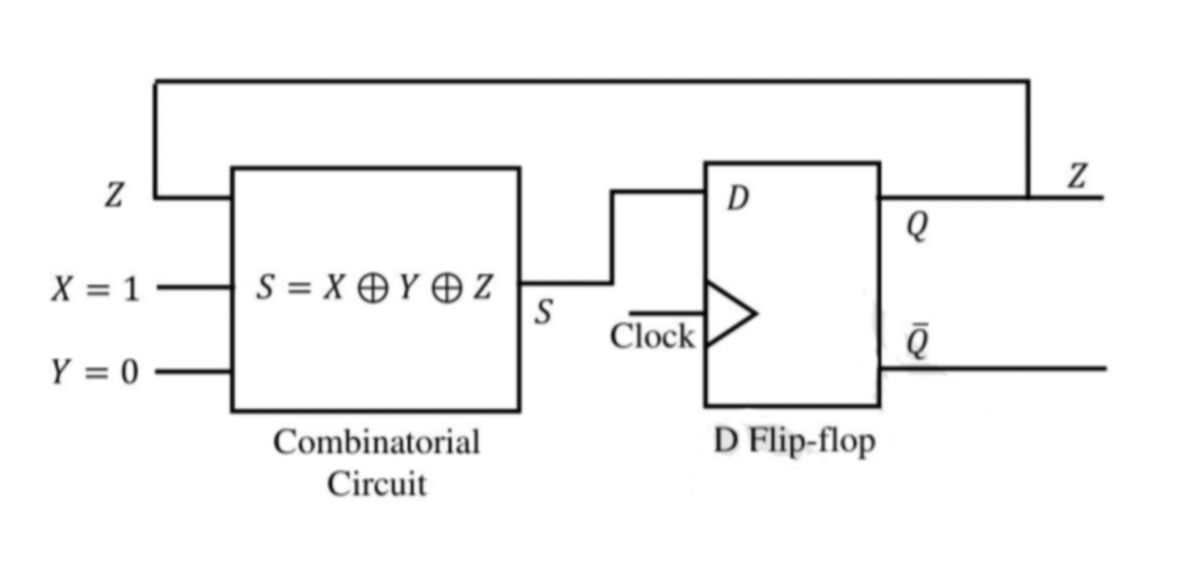
\includegraphics[width=0.35\textwidth]{IMG-20241021-WA0008   }
 \caption{\label{fig:Gates}}
 \end {figure}
\section{COMPONENTS}
The required components list is given in Table: I. Flip-flop IC 7474 diagram is shown in Fig.2.
\begin{figure}[h]
\centering
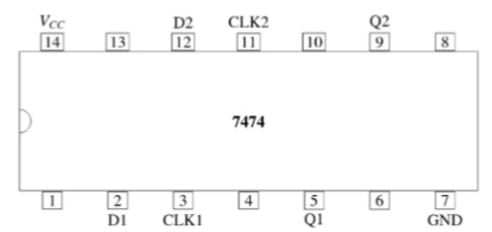
\includegraphics[width=0.35\textwidth]{IMG-20241021-WA0003}
\caption{\label{fig:Gates}}
\end{figure}
 \begin{table} [htbp]
\centering
\begin{tabular}{| c | c | c |} \hline
Components & Value & Quantity \\\hline
IC & 7474 & 1 \\ \hline
LEDs &  & 1 \\ \hline
Arduino & UNO & 1 \\ \hline
Jumper Wires &  & 10 \\ \hline
Breadboard & & 1 \\ 
\hline
\end{tabular}
\vspace{0.1cm}
\caption{\label{tab:widgets}}
\end{table}
\section{PROCEDURE}
Make the connections between Arduino and 7474 as per the Table: II.
 \begin{table}[htbp]                                       
\centering                                                          
\begin{tabular}{| c | c |} \hline                                
	\textbf{Arduino Pin} & \textbf{7474}  \\\hline 
D5 & 2  \\ \hline                                             
D6 &  3 \\ \hline                                               
D4 & 5 \\ \hline                                           
5 V  & 14 \\ \hline                                        
gnd  & 7 \\                                                   
\hline                                                               
\end{tabular}                                                        
\vspace{0.1cm}                                                       
\caption{\label{tab:widgets}}                                       
\end{table}
\section{RESULTS}
Download the cod given in the link below and execute them to see the output as shown in Fig.2 by placing the LED at the output pin of 7474 IC. 
https://github.com/rajib05ra/FWC-Assignments/tree/main/Assignment%20IDE/IDE%20Code%20run/src
\begin{figure}[h] 
	\centering 
	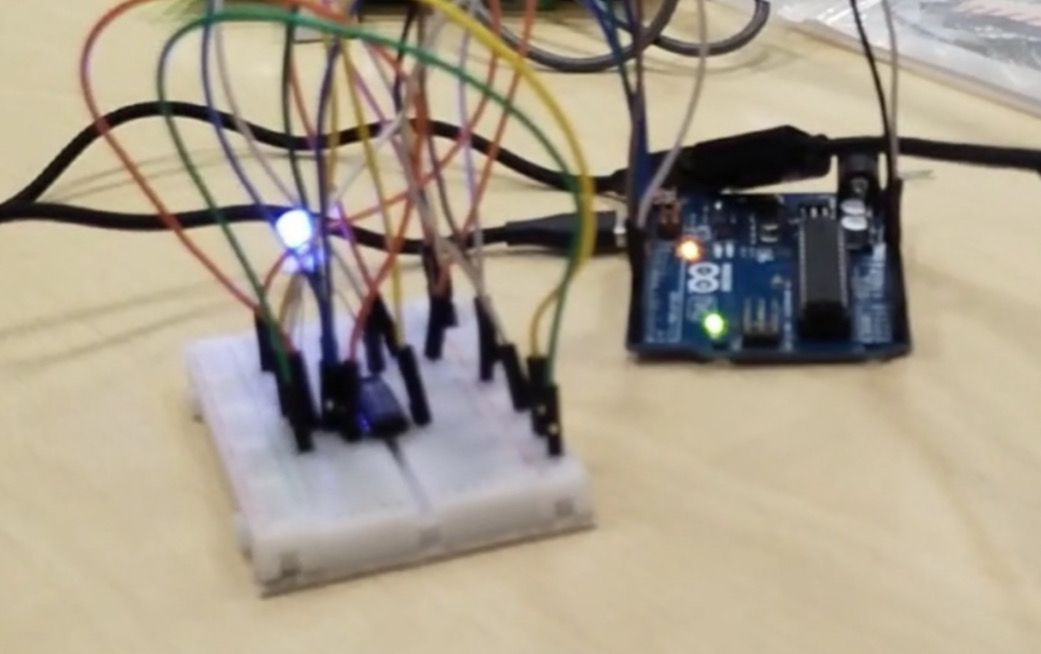
\includegraphics[width=0.35\textwidth]{IMG-20241021-WA0009}
	\caption{\label{fig:Gates}}    
\end{figure}
\section{CONCLUSION}
The D-Flip Flop is a good application in order to use it for registers. Here, the sequential circuit is combined with the combinational circuit of XOR gates to get the output. Therefore, we can design several circuits and can be implemented using Arduino and Platformio.
\end{document}
